\documentclass[12pt]{article}

\usepackage{fullpage}
\usepackage{graphicx}
\usepackage{amssymb}
\usepackage{fancyvrb}
\usepackage{amsmath}
\usepackage{setspace}
\usepackage[margin=1in]{geometry}
\usepackage[resetlabels,labeled]{multibib}
\usepackage{wrapfig}

\newcites{New}{The other list}

\begin{document}

\begin{wrapfigure}{r}{0.4\textwidth}
  \begin{center}
    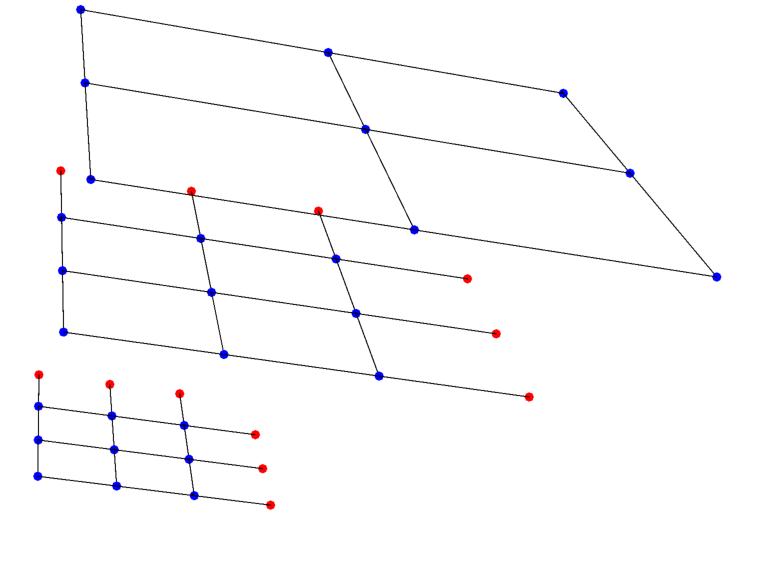
\includegraphics[scale=0.4]{nsfpic.pdf}
  \end{center}
  \caption{\footnotesize{Blue:grid points to be calculated. Red:fixed boundary estimates}}
\end{wrapfigure}
    
    
    Consider $\bigtriangledown \epsilon \bigtriangleup u = f$, discretization by the spectral method and solved using multigrid.
    
    Discretizing the domain by the Spectral Method and solving using multigrid yields a solution with a fourier representation that is arbitrarily accurate up to k coefficients (when using, e.g. gmres to find unknowns). To get higher accuracy, one can refine the grid further. Using an initial guess for some of the unknowns from the coarse grid, low frequency errors are still small, but high frequency errors are possibly high. 
    
    Now consider the buffer zone introduced by segmental refinement, which can be represented as a new grid with two boundary conditions encoding the error by this buffer zone. The boundary will thus be functions with fourier coefficients of k or greater since the coarser grid was ~accurate up to k coefficients. 
    
    We must demonstrate that the solution to this grid with boundary values of frequency k will decay to discretization error by the time it leaves the buffer zone. On this finer grid, then, we will have error introduced by discretization of frequency 2k or higher, combined with the error that is introduced by the buffer zone and decays to discretization error. Overall, this function will still be accurate up to coefficients of 2k.
    
    Inductively, we will see that at every level of refinement, we get accuracy up to coefficients of $(2^n) k$ because at the previous level, we had $(2^{n-1}) k$ orders of accuracy.
    
    Remark: We must show that the fourier coefficients of solutions to these laplace equations decay at a certain rate in order to show that solving up to $(2^{n})$ coefficients will yield a sum that decays very quickly as we take a shorter and shorter tail of the sum. Each of the functions Sin(k x) exist on the buffer zone boundary. Even if they decay at a certain rate, we must also show that the sum of these functions decays and in order to show this, there is undoubtedly a bound on the sum of their coefficients. 
    
    
    
    
    
    
    
    

% \textbf{Intellectual Merit:} 
% We will find an analytical estimate for the decay of error introduced by segmental refinement as a function of wave number and strength of the boundary value perturbation. Also, we will provide a software framework for limited memory hierarchical algorithms. 
% %analytical estimate for the decay of error away from the boundary as a function of the wave number and strength of the boundary value perturbation. introduced error decays away from boundary. we will provide a software framework for limited memory hierarchical algorithms. 

% \textbf{Broader Impact:}
% A pillar of my research would be the implementation of the algorithm in open-source form such that a researcher, even one outside of the field of mathematics, could use.This would make SRMG available to experts of fields outside of mathematics without access to a computational expert as a collaborator, who still need to compute solutions to large problems. The nature of the algorithm increases the scale of problems that our strongest supercomputers can solve, as well as the scale of problems solvable on a personal computer. This makes more problems accessible to all scales of researchers, from large organizations with access to supercomputers to individual researchers without access to these resources. 

%\textbf{Need: citation that software grows quickly, flops per unknown, problems solved with multigrid, }

%Consider a laptop capable of 10^9 operations per second. An upper estimate of the computational complexity of this problem is 500 to 10^2 operations required for each unknown. Consider 10% performance of computer. 10^2*10^12 10^(9) = 10^5 = 25 hours.  

{\footnotesize
\bibliographystyle{IEEEtran}
\bibliography{IEEEabrv,references}

\bibliographystyleNew{IEEEtran}
\bibliographyNew{IEEEabrv, references}
}
\end{document}


\title{Multiple Bibliographies with \texttt{multibib}}
\author{LianTze Lim}
\date{}


\usepackage[resetlabels,labeled]{multibib}

%% The new list's label is "New" and will be titled "The other list".
%% To put cites into this list, use \citeNew.
\newcites{New}{The other list}

\begin{document}

\maketitle

\cite{mydog} and \cite{url} were published later than

\bibliographystyle{plain}
\bibliography{references}

\bibliographystyleNew{plain}
\bibliographyNew{references}

\end{document}

1. Aitken's array http://oeis.org/search?q=1%2C1%2C+2%2C+2%2C+3%2C+5%2C+5&language=english&go=Search
2. https://en.wikipedia.org/wiki/Stirling%27s_approximation
3. http://ubuntuforums.org/showthread.php?t=1244186
4.It appears Newton deserves majority credit. Rhapson may have just simplified things.  It appears many people were https://en.wikipedia.org/wiki/Newton%27s_method#History
5. https://en.wikipedia.org/wiki/Leonid_Kantorovich
6. http://www.iue.tuwien.ac.at/phd/entner/node9.html
7. https://en.wikipedia.org/wiki/Special:Contributions/Jrt54 
7. https://en.wikipedia.org/w/index.php?title=Latent_semantic_indexing&diff=prev&oldid=682352132